% ============================================================
%  DISCOVERY CURRICULUM — Journey 1, Module 5
%  "Growth and Recursion"
%  Compile with: pdflatex J1_M5.tex  (run twice for references)
% ============================================================

\documentclass[12pt, a4paper]{article}

\usepackage[a4paper, top=2.8cm, bottom=2.8cm, left=3.0cm, right=2.5cm, includeheadfoot, headheight=15pt]{geometry}
\usepackage{amsmath, amsthm}
\usepackage[charter, cal=cmcal]{mathdesign}
\usepackage[scaled=0.92]{helvet}
\usepackage{xcolor}
\usepackage{tcolorbox}
\tcbuselibrary{skins, breakable, theorems}
\usepackage{enumitem}
\usepackage{graphicx}
\usepackage{tikz}
\usetikzlibrary{arrows.meta, positioning, calc}
\usepackage{pgfplots}
\pgfplotsset{compat=1.18}
\usepackage{booktabs}
\usepackage{array}
\usepackage{fancyhdr}
\usepackage{titlesec}
\usepackage{parskip}
\usepackage{microtype}
\usepackage{hyperref}
\hypersetup{colorlinks=true, linkcolor=NavyBlue, urlcolor=NavyBlue}

% ── Colours ─────────────────────────────────────────────────
\definecolor{NavyBlue}{HTML}{1E3A8A}
\definecolor{MidBlue}{HTML}{2E6DA4}
\definecolor{Gold}{HTML}{D97706}
\definecolor{LightBlue}{HTML}{EFF6FF}
\definecolor{LightGold}{HTML}{FEF3C7}
\definecolor{DarkGrey}{HTML}{334155}
\definecolor{BoxGreen}{HTML}{F0FDF4}
\definecolor{SoftRed}{HTML}{FFF1F2}
\definecolor{SidebarGrey}{HTML}{F8FAFC}

% ── Section formatting ───────────────────────────────────────
\titleformat{\section}{\Large\bfseries\color{NavyBlue}}{}{0em}{}[{\color{MidBlue}\vspace{2pt}\rule{\linewidth}{1.5pt}}]
\titleformat{\subsection}{\large\bfseries\color{MidBlue}}{}{0em}{}
\titleformat{\subsubsection}{\normalsize\bfseries\color{Gold}}{}{0em}{}

% ── Header / Footer ─────────────────────────────────────────
\pagestyle{fancy}
\fancyhf{}
\fancyhead[L]{\small\color{DarkGrey}\textit{Discovery Curriculum}}
\fancyhead[R]{\small\color{DarkGrey}\textit{Journey 1 $\cdot$ Module 5}}
\fancyfoot[C]{\small\color{MidBlue}\thepage}
\renewcommand{\headrulewidth}{0.4pt}

% ── Environments (tcolorbox Unification) ─────────────────────

% Puzzle box — opening problem
\newtcolorbox{puzzlebox}[1][]{
  enhanced, breakable,
  colback=NavyBlue!5, colframe=NavyBlue,
  boxrule=0pt, leftrule=2.5pt,
  sharp corners,
  left=12pt, right=10pt, top=10pt, bottom=10pt,
  before skip=14pt, after skip=10pt,
  #1
}

% Discovery box — moment of crystallisation
\newtcolorbox{discoverybox}[1][]{
  enhanced, breakable,
  colback=LightGold, colframe=Gold,
  boxrule=0pt, leftrule=2.5pt,
  sharp corners,
  left=12pt, right=10pt, top=10pt, bottom=10pt,
  before skip=14pt, after skip=10pt,
  #1
}

% Name box — formal definition reveal
\newtcolorbox{namebox}[1][]{
  enhanced, breakable,
  colback=LightBlue, colframe=MidBlue,
  boxrule=0.8pt,
  arc=4pt,
  left=12pt, right=10pt, top=10pt, bottom=10pt,
  before skip=14pt, after skip=10pt,
  #1
}

% Reflection box
\newtcolorbox{reflectionbox}[1][]{
  enhanced, breakable,
  colback=BoxGreen, colframe=DarkGrey!35,
  boxrule=0.8pt,
  arc=4pt,
  left=12pt, right=10pt, top=10pt, bottom=10pt,
  before skip=14pt, after skip=10pt,
  #1
}

% Thought provocation — inline philosophical aside
\newtcolorbox{thought}[1][]{
  enhanced, breakable,
  colback=SidebarGrey, colframe=Gold,
  boxrule=0pt, leftrule=1.5pt,
  sharp corners,
  left=10pt, right=10pt, top=7pt, bottom=7pt,
  before skip=10pt, after skip=10pt,
  #1
}

% Problem counter
\newcounter{problem}
\newenvironment{problem}[1][]{%
  \refstepcounter{problem}%
  \par\vspace{6pt}%
  \noindent\textbf{\color{MidBlue}Problem \theproblem}%
  \ifx&#1&\else\ \textit{(#1)}\fi\textbf{.}\enskip
}{\par\vspace{4pt}}

% Deep problem counter
\newcounter{deepproblem}
\newenvironment{deepproblem}[1][]{%
  \refstepcounter{deepproblem}%
  \par\vspace{6pt}%
  \noindent\textbf{\color{NavyBlue}$\bigstar$\ Deep Problem \thedeepproblem}%
  \ifx&#1&\else\ \textit{(#1)}\fi\textbf{.}\enskip
}{\par\vspace{4pt}}

% Exercise counter
\newcounter{exercise}
\newenvironment{exercise}[1][]{%
  \refstepcounter{exercise}%
  \par\vspace{6pt}%
  \noindent\textbf{\color{Gold}Exercise \theexercise}%
  \ifx&#1&\else\ \textit{(#1)}\fi\textbf{.}\enskip
}{\par\vspace{4pt}}

\begin{document}
% ============================================================

% ── Cover ───────────────────────────────────────────────────
\thispagestyle{empty}
\begin{center}
{\small\color{MidBlue}\textbf{DISCOVERY CURRICULUM}\quad$\cdot$\quad\textbf{JOURNEY 1: REPRESENTATION}}

\vspace{0.6cm}
{\color{NavyBlue}\rule{\linewidth}{2pt}}
\vspace{0.5cm}

{\Huge\bfseries\color{NavyBlue}Module 5}\\[0.3cm]
{\LARGE\bfseries\color{MidBlue}Growth and Recursion}\\[0.4cm]
{\color{Gold}\rule{0.4\linewidth}{1.2pt}}\\[0.4cm]
{\large\itshape\color{DarkGrey}
What is the most natural rate of growth?\\[0.15cm]
And why does the same strange number keep appearing everywhere?}

\vspace{1cm}
\begin{tabular}{rl}
\color{DarkGrey}\textbf{Journey}           & Journey 1 --- Representation \\[4pt]
\color{DarkGrey}\textbf{Module}            & 5 of 6 \\[4pt]
\color{DarkGrey}\textbf{Prerequisites}     & Modules 1--4 (functions, sequences, limits) \\[4pt]
\color{DarkGrey}\textbf{You will discover} & The number $e$, exponential functions, logarithms, continuous growth \\[4pt]
\color{DarkGrey}\textbf{Format}            & 8 problems $+$ 3 deep problems $\approx$ 12--14 pages \\
\end{tabular}

\vspace{1cm}
{\color{NavyBlue}\rule{\linewidth}{2pt}}
\end{center}

\vspace{0.6cm}

\noindent\textbf{Recap of Module 4.}
In Module~4 you discovered that sequences can grow geometrically, converge to limits, and --- in the case of recursive rules --- exhibit behaviour ranging from steady convergence to complete chaos. The Fibonacci sequence revealed that its ratio converges to a specific algebraic number, the golden ratio, derivable from the recursion itself.

\medskip
This module follows a single thread: \emph{what is the most natural way for a quantity to grow?} The answer leads to one of the most remarkable numbers in mathematics --- a number that appears in compound interest, population dynamics, radioactive decay, the normal distribution, complex numbers, and the deepest identity in all of mathematics. We will not name it until we have discovered it.

\newpage

% ============================================================
\section{Part 1 \texorpdfstring{---}{--} The Puzzle}
% ============================================================

\begin{puzzlebox}
\textbf{The Opening Puzzle.}

A bank offers you an interest rate of 100\% per year. You invest 1 unit of currency.

\begin{itemize}
  \item If interest is paid \textbf{once} at year end: you have $1 + 1 = 2$.
  \item If paid \textbf{twice} (50\% each half-year): you have $\left(1 + \tfrac{1}{2}\right)^2 = 2.25$.
  \item If paid \textbf{four times} (25\% each quarter): you have $\left(1 + \tfrac{1}{4}\right)^4 \approx 2.4414$.
  \item If paid \textbf{twelve times} monthly: $\left(1 + \tfrac{1}{12}\right)^{12} \approx 2.6130$.
  \item If paid \textbf{365 times} daily: $\left(1 + \tfrac{1}{365}\right)^{365} \approx 2.7146$.
\end{itemize}

\medskip
\textbf{Question 1.} What happens as the number of compounding periods $n$ grows without bound? Does this sequence $\left(1 + \tfrac{1}{n}\right)^n$ converge or diverge?

\textbf{Question 2.} Compute $\left(1 + \tfrac{1}{n}\right)^n$ for $n = 100,\; 1000,\; 10{,}000,\; 100{,}000$. What value does it appear to approach? Write down as many decimal places as you can.

\textbf{Question 3.} Why should there be a finite limit at all? What is special about the growth process that produces it?
\end{puzzlebox}

\medskip
You have just stumbled upon one of the most important numbers in mathematics. It is irrational, transcendental, and appears in contexts that seem to have nothing to do with interest rates. Before we name it, let us understand why it had to exist.

\begin{thought}
\textbf{What does ``continuous'' growth mean?}
The compounding puzzle is really asking: what happens when growth is not applied in discrete steps, but continuously, at every instant? The interest rate is 100\%, but it is applied infinitely often in infinitely small doses. The limiting process you are computing is the mathematical formalisation of growth that is happening \emph{all the time}, without interruption. This idea --- growth as a continuous process rather than a sequence of discrete jumps --- is the conceptual bridge between the sequences of Module~4 and the calculus of Journey~2. The number you are approaching is, in a precise sense, the value of ``1 unit growing continuously at rate 1 for 1 unit of time.''
\end{thought}

% ============================================================
\section{Part 2 \texorpdfstring{---}{--} Exploration}
% ============================================================

\subsection{Step 1: Discovering the limit}

\begin{problem}
\label{prob:e_limit}
Let $a_n = \left(1 + \dfrac{1}{n}\right)^n$.

\begin{enumerate}[label=(\alph*), topsep=2pt]
  \item Compute $a_n$ for $n = 1, 2, 5, 10, 100, 1000$. Record at least 5 decimal places.
  \item Show that the sequence $(a_n)$ is \emph{increasing}: verify $a_2 > a_1$, $a_3 > a_2$, and argue why this should continue.
  \item Show that the sequence is \emph{bounded above} by 3: argue that $\left(1+\tfrac{1}{n}\right)^n < 3$ for all $n$. \textit{Hint: use the binomial theorem and compare with the series $1 + 1 + \tfrac{1}{2!} + \tfrac{1}{3!} + \cdots$}
  \item An increasing sequence that is bounded above must converge (this is a fundamental theorem about real numbers --- can you see why it must be true?). What does this tell you about $(a_n)$?
  \item Now compute $b_n = \left(1 + \dfrac{1}{n}\right)^{n+1}$. Is this sequence increasing or decreasing? Does it converge to the same limit?
\end{enumerate}
\end{problem}

\begin{problem}
\label{prob:e_series}
Expand $\left(1 + \dfrac{1}{n}\right)^n$ using the binomial theorem:
\[
\left(1 + \frac{1}{n}\right)^n
= \sum_{k=0}^{n} \binom{n}{k} \frac{1}{n^k}
= \sum_{k=0}^{n} \frac{n(n-1)(n-2)\cdots(n-k+1)}{k!\; n^k}.
\]
\begin{enumerate}[label=(\alph*), topsep=2pt]
  \item Show that $\dfrac{n(n-1)\cdots(n-k+1)}{n^k} = \left(1 - \dfrac{1}{n}\right)\left(1-\dfrac{2}{n}\right)\cdots\left(1-\dfrac{k-1}{n}\right)$.
  \item As $n \to \infty$, each factor $\left(1 - \dfrac{j}{n}\right) \to 1$. What does each term of the sum approach?
  \item Taking the limit term-by-term (which requires justification we will not fully supply here), show that
  \[
    \lim_{n\to\infty}\left(1+\frac{1}{n}\right)^n = \sum_{k=0}^{\infty} \frac{1}{k!} = 1 + 1 + \frac{1}{2} + \frac{1}{6} + \frac{1}{24} + \cdots
  \]
  \item Compute the partial sums of $\sum_{k=0}^{\infty} \frac{1}{k!}$ up to $k = 8$. How close are you to the limit?
\end{enumerate}
\end{problem}

\subsection{Step 2: The exponential function}

\begin{problem}
\label{prob:exp_properties}
Define $f(x) = \left(1 + \dfrac{x}{n}\right)^n$ as $n \to \infty$ for a general real number $x$.
\begin{enumerate}[label=(\alph*), topsep=2pt]
  \item Compute this limit for $x = 2$ by evaluating $\left(1 + \frac{2}{n}\right)^n$ for large $n$.
  \item Compute for $x = -1$. What do you get? Does it make sense that growth at rate $-1$ gives a decay?
  \item Argue (informally) that the limit for general $x$ should be $\displaystyle\sum_{k=0}^{\infty} \frac{x^k}{k!}$.
  \item Let $E(x) = \displaystyle\sum_{k=0}^{\infty} \frac{x^k}{k!}$. Compute $E(0)$. Compute $E(1)$.
  \item Prove algebraically that $E(x) \cdot E(y) = E(x+y)$ using the series definition. \textit{Hint: multiply the two series and collect terms by total power.}
  \item What does the identity $E(x) \cdot E(y) = E(x+y)$ say in plain language about this function?
\end{enumerate}
\end{problem}

\begin{thought}
\textbf{The defining property of exponential growth.}
The identity $E(x+y) = E(x) \cdot E(y)$ is not just a formula --- it is a characterisation. It says: \emph{adding inputs corresponds to multiplying outputs}. This is exactly what it means for growth to be exponential. If you grow for time $x$ and then for time $y$, the total growth factor is the product of the individual growth factors. This is the mathematical signature of compound interest, population growth, radioactive decay, and the spread of disease.

Any function satisfying $f(x+y) = f(x) \cdot f(y)$ with $f$ continuous must be of the form $f(x) = a^x$ for some base $a > 0$. (Compare this with the functional equation $f(x+y) = f(x) + f(y)$ from Deep Problem~1 of Module~1, which forces $f(x) = cx$. The multiplicative version forces exponential growth. Additive equation, linear function. Multiplicative equation, exponential function. The symmetry is beautiful.)
\end{thought}

\begin{problem}
\label{prob:exp_graph}
The function $E(x) = e^x$ where $e = E(1) = \sum_{k=0}^{\infty} \frac{1}{k!} \approx 2.71828\ldots$
\begin{enumerate}[label=(\alph*), topsep=2pt]
  \item Plot $e^x$ for $x \in [-3, 3]$ by computing values at $x = -3, -2, -1, 0, 0.5, 1, 1.5, 2, 3$.
  \item At $x = 0$, the slope of $e^x$ appears to be 1. Estimate the slope at $x = 1$ and at $x = 2$ by computing $\frac{e^{x+h} - e^x}{h}$ for small $h = 0.001$. What do you notice?
  \item The slope of $e^x$ at any point $x$ is $e^x$ itself. This is \emph{the} defining property of $e^x$ among all exponential functions. Why is this remarkable? What does it mean for a function to be its own rate of change?
  \item Compare $2^x$, $e^x$, and $3^x$ on the same axes. At $x = 0$, estimate the slopes of $2^x$ and $3^x$. Where do they fall relative to $e^x$?
\end{enumerate}
\end{problem}

\begin{center}
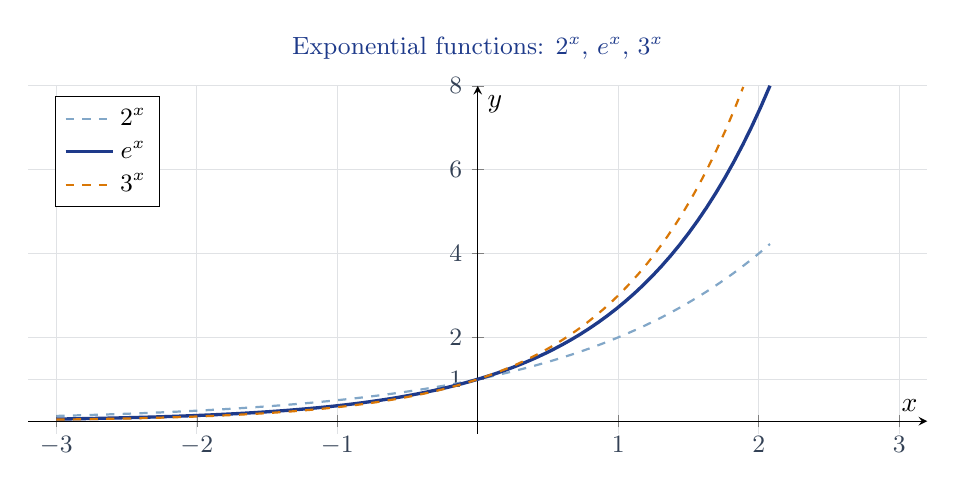
\begin{tikzpicture}
\begin{axis}[
  width=13cm, height=6cm,
  axis lines=center,
  xlabel={$x$}, ylabel={$y$},
  xmin=-3.2, xmax=3.2, ymin=-0.3, ymax=8,
  xtick={-3,-2,-1,1,2,3},
  ytick={1,2,4,6,8},
  tick label style={font=\small, color=DarkGrey},
  grid=major, grid style={DarkGrey!15},
  legend pos=north west,
  legend style={font=\small},
  title={\small\color{NavyBlue}Exponential functions: $2^x$, $e^x$, $3^x$},
]
\addplot[MidBlue!60, thick, dashed, domain=-3:2.08, samples=80] {2^x};
\addplot[NavyBlue, very thick, domain=-3:2.08, samples=80] {e^x};
\addplot[Gold, thick, dashed, domain=-3:1.89, samples=80] {3^x};
\addlegendentry{$2^x$}
\addlegendentry{$e^x$}
\addlegendentry{$3^x$}
\end{axis}
\end{tikzpicture}
\end{center}

\subsection{Step 3: The inverse --- logarithms}

\begin{problem}
\label{prob:log}
Since $e^x$ is a bijection from $\mathbb{R}$ to $(0, \infty)$ (verify this), it has an inverse function.
\begin{enumerate}[label=(\alph*), topsep=2pt]
  \item If $e^x$ maps $\mathbb{R} \to (0,\infty)$, the inverse maps $(0,\infty) \to \mathbb{R}$. Call it $\ln$. What does $\ln(e^x) = x$ and $e^{\ln y} = y$ say in plain language?
  \item Using the identity $e^{x+y} = e^x \cdot e^y$, derive the identity $\ln(ab) = \ln a + \ln b$. This is the law that made logarithms the most important computational tool before electronic calculators.
  \item Derive $\ln(a^r) = r \ln a$.
  \item A population of bacteria doubles every 3 hours. Starting from 500 bacteria, after how many hours will there be 10{,}000? Set up the equation and solve it using logarithms.
  \item Carbon-14 has a half-life of 5730 years. A bone fragment contains 30\% of its original Carbon-14. How old is the bone? Set up and solve.
\end{enumerate}
\end{problem}

\begin{thought}
\textbf{Why logarithms mattered so much.}
Before 1614, multiplication of large numbers was extraordinarily tedious --- multiplying two 8-digit numbers required dozens of arithmetic operations and invited error. Then \textbf{John Napier} published his table of logarithms. Because $\log(ab) = \log a + \log b$, \emph{multiplication becomes addition}. A navigator or astronomer could look up two logarithms, add them, and look up the result. For two centuries, logarithm tables were the most important computational technology in the world. They made the scientific revolution possible. Kepler used them to compute planetary orbits. Newton used them. Every serious scientist and engineer until the 1970s spent hours learning to use them fluently.

Then the pocket calculator was invented and logarithm tables became obsolete almost overnight. But the concept of a logarithm did not become obsolete. It reappears in information theory (the number of bits to encode a message), in entropy (the disorder of a system), in complexity theory (the efficiency of algorithms), and in every part of science that deals with quantities spanning many orders of magnitude. The tool died; the idea lives.
\end{thought}

\subsection{Step 4: Growth rates and comparison}

\begin{problem}
\label{prob:growth_compare}
Different functions grow at very different rates. Understanding which functions dominate which is essential in algorithm analysis, physics, and statistics.
\begin{enumerate}[label=(\alph*), topsep=2pt]
  \item Compute and compare at $n = 10, 100, 1000$:
  \[
    \ln n, \quad \sqrt{n}, \quad n, \quad n^2, \quad 2^n, \quad n!
  \]
  \item Arrange these six functions in order of growth rate (slowest to fastest) for large $n$.
  \item For each pair of adjacent functions in your ordering, compute their ratio at $n = 100$ and $n = 1000$. What happens to the ratio as $n$ grows?
  \item An algorithm takes $n^2$ steps. A second algorithm takes $2^n$ steps. For which values of $n$ is the first faster? For which is it slower? At what point does the second algorithm become completely impractical, say taking more than $10^{20}$ steps?
  \item Stirling's approximation says $n! \approx \sqrt{2\pi n}\left(\frac{n}{e}\right)^n$ for large $n$. Check this for $n = 10$ and $n = 20$ by computing both sides. What does the presence of $e$ and $\pi$ in this approximation suggest to you?
\end{enumerate}
\end{problem}

\begin{problem}
\label{prob:natural_growth}
A quantity $Q(t)$ grows so that its rate of change at every instant is proportional to its current size:
\[
  \frac{Q(t+h) - Q(t)}{h} \approx k \cdot Q(t) \quad \text{for small } h.
\]
\begin{enumerate}[label=(\alph*), topsep=2pt]
  \item This is the continuous analogue of geometric growth. If $Q(0) = Q_0$, argue (using the compounding idea) that $Q(t) = Q_0 e^{kt}$.
  \item Verify: if $Q(t) = Q_0 e^{kt}$, then doubling time $T_2$ satisfies $kT_2 = \ln 2$. Use this to find the doubling time for a bacterial population growing at $k = 0.2$ per hour.
  \item Radioactive decay satisfies the same law with $k < 0$. Express the half-life $T_{1/2}$ in terms of $k$.
  \item A rumour spreads through a school of 1000 students. At time $t = 0$, 10 students know it. Assume exponential spread with $k = 0.5$ per hour. When do 500 students know? When do 999 know?
  \item At some point exponential growth always breaks down as a model of reality. List three specific mechanisms that would cause real population growth to slow down, and explain which mathematical model you think might replace the pure exponential.
\end{enumerate}
\end{problem}

\begin{thought}
\textbf{The unreasonable speed of exponential growth.}
In 1859, Thomas Austin released 24 rabbits in Victoria, Australia. By 1920, there were an estimated 10 billion. The mathematics is straightforward: exponential growth with a doubling time of about 1 year. Within 50 years, the invasion had caused catastrophic ecological damage across an entire continent. Yet people approved the release of 24 rabbits. The failure was not one of malice but of intuition: human beings are very poor at internalising exponential growth. The same failure appears in the spread of diseases, the growth of national debt compounded annually, the proliferation of nuclear weapons, and the accumulation of carbon in the atmosphere. The mathematics is not complicated. The intuition, apparently, is.
\end{thought}

\begin{problem}
\label{prob:euler_identity}
We end with the most remarkable formula in mathematics. It connects five fundamental constants.

\medskip
Consider the function $E(x) = \displaystyle\sum_{k=0}^{\infty} \frac{x^k}{k!}$, but now allow $x$ to be a complex number. In particular, let $x = i\theta$ where $i^2 = -1$ and $\theta$ is real.

\begin{enumerate}[label=(\alph*), topsep=2pt]
  \item Compute the first six terms of $E(i\theta) = \sum_{k=0}^{\infty} \frac{(i\theta)^k}{k!}$. Use $i^2 = -1$, $i^3 = -i$, $i^4 = 1$, and so on.
  \item Separate the real and imaginary parts of your sum. You should recognise two familiar series.
  \item What famous formula have you just derived?
  \item Set $\theta = \pi$. What do you get? Simplify.
  \item The result $e^{i\pi} + 1 = 0$ connects $e$, $i$, $\pi$, $1$, and $0$ --- the five most fundamental constants of mathematics --- in a single equation. Does the existence of this identity feel like a discovery or a coincidence to you? Write two sentences.
\end{enumerate}
\end{problem}

\begin{thought}
\textbf{Euler's identity and the question of mathematical beauty.}
In surveys of mathematicians, Euler's identity $e^{i\pi} + 1 = 0$ is consistently voted the most beautiful equation in mathematics. But what does it mean for a mathematical statement to be \emph{beautiful}? The physicist Richard Feynman called it ``the most remarkable formula in mathematics.'' The mathematician G.~H.\ Hardy wrote that beauty is the first test: there is no permanent place in mathematics for ugly mathematics. These are aesthetic judgements, not logical ones. Mathematics is sometimes presented as a purely logical enterprise, stripped of human feeling. But mathematicians experience surprise, delight, and disappointment. They have favourite theorems. They describe proofs as clumsy or elegant. Whether mathematics is discovered or invented, whether beauty is a guide to truth or a trap --- these questions have no clean answers. They are worth sitting with.
\end{thought}

% ============================================================
\section{Part 3 \texorpdfstring{---}{--} Discovery}
% ============================================================

\begin{discoverybox}
\textbf{What have we built?}

This module followed a single thread from compound interest to one of the deepest formulas in all of mathematics.

\medskip
\textbf{First.} The limit $e = \lim_{n\to\infty}\left(1 + \tfrac{1}{n}\right)^n$ is forced into existence by the compounding process. It is not an arbitrary constant --- it is the value of continuous growth at unit rate.

\medskip
\textbf{Second.} The function $e^x$ is characterised by a remarkable property: it is its own rate of change. No other base has this property. This is why $e$ is the ``natural'' base for exponential functions.

\medskip
\textbf{Third.} The inverse function $\ln x$ turns multiplication into addition, which is both computationally powerful and theoretically profound. It reappears in information theory, entropy, and complexity.

\medskip
\textbf{Fourth.} The series definition $e^x = \sum x^k/k!$ extends naturally to complex numbers and, when evaluated at $x = i\pi$, yields an identity connecting five fundamental constants.

\medskip
\textbf{Before reading on:} The property ``$e^x$ is its own derivative'' will be made precise in Journey~2. For now: if a quantity $Q$ satisfies $Q' = kQ$ (its rate of change is proportional to itself), can you guess what $Q(t)$ must be? What initial condition determines it uniquely?
\end{discoverybox}

% ============================================================
\section{Part 4 \texorpdfstring{---}{--} Naming the Ideas}
% ============================================================

\begin{namebox}
\textbf{The number $e$ and the exponential function.}

The number $e$ is defined by
\[
  e \;=\; \lim_{n\to\infty}\left(1+\frac{1}{n}\right)^n \;=\; \sum_{k=0}^{\infty}\frac{1}{k!} \;=\; 1 + 1 + \frac{1}{2} + \frac{1}{6} + \frac{1}{24} + \cdots \;\approx\; 2.71828\ldots
\]
It is irrational (proved by Euler, 1737) and transcendental (proved by Hermite, 1873).

\medskip
The \textbf{exponential function} $\exp(x) = e^x$ is the unique function satisfying
\[
  \frac{d}{dx}e^x = e^x \qquad \text{and} \qquad e^0 = 1.
\]
Equivalently: $e^{x+y} = e^x \cdot e^y$ for all real (and complex) $x, y$.
\end{namebox}

\begin{namebox}
\textbf{The natural logarithm.}

The \textbf{natural logarithm} $\ln : (0,\infty) \to \mathbb{R}$ is the inverse of $e^x$:
\[
  \ln(e^x) = x \quad \forall\, x \in \mathbb{R}, \qquad e^{\ln y} = y \quad \forall\, y > 0.
\]
Key identities: $\ln(ab) = \ln a + \ln b$; \quad $\ln(a^r) = r\ln a$; \quad $\ln 1 = 0$; \quad $\ln e = 1$.

The natural logarithm was introduced by \textbf{John Napier} (1614) and systematised by \textbf{Leonhard Euler}.
\end{namebox}

\begin{namebox}
\textbf{Euler's formula and identity.}

For any real $\theta$:
\[
  e^{i\theta} = \cos\theta + i\sin\theta \qquad \textbf{(Euler's formula)}
\]
Setting $\theta = \pi$:
\[
  e^{i\pi} + 1 = 0 \qquad \textbf{(Euler's identity)}
\]
This follows from the power series $e^x = \sum x^k/k!$ extended to complex $x$, and the series representations $\cos\theta = \sum(-1)^k\theta^{2k}/(2k)!$ and $\sin\theta = \sum(-1)^k\theta^{2k+1}/(2k+1)!$.
\end{namebox}

% ============================================================
\section{Part 5 \texorpdfstring{---}{--} Deep Problems}
% ============================================================

\begin{deepproblem}[Irrationality and transcendence]
\begin{enumerate}[label=(\alph*)]
  \item Prove that $e$ is irrational. \textit{Hint: assume $e = p/q$ for integers $p, q > 0$. Consider $q!\left(e - \sum_{k=0}^{q}\frac{1}{k!}\right)$ and show it is simultaneously a positive integer and strictly less than 1.}
  \item A number is \textbf{algebraic} if it is the root of a polynomial with integer coefficients; it is \textbf{transcendental} otherwise. Show that $\sqrt{2}$ is algebraic. Is $\sqrt{2} + \sqrt{3}$ algebraic?
  \item Liouville showed in 1844 that transcendental numbers exist by constructing one explicitly: $\sum_{k=1}^{\infty} 10^{-k!}$. Explain why this number cannot be a root of any polynomial with integer coefficients.
  \item Hermite proved $e$ is transcendental in 1873. Lindemann proved $\pi$ is transcendental in 1882. As a consequence, which ancient geometric construction was finally proved impossible, and why?
\end{enumerate}
\end{deepproblem}

\begin{deepproblem}[The Gaussian and the normal distribution]
The function $f(x) = e^{-x^2}$ appears throughout probability and physics.
\begin{enumerate}[label=(\alph*)]
  \item Plot $f(x) = e^{-x^2}$ for $x \in [-3,3]$. Describe its shape. Where is it maximised? Where does it decay fastest?
  \item One of the most surprising results in analysis is $\displaystyle\int_{-\infty}^{\infty} e^{-x^2}\,dx = \sqrt{\pi}$. This means $\pi$ appears in the area under a bell curve. Verify numerically that the partial integral $\int_{-3}^{3} e^{-x^2}\,dx$ is close to $\sqrt{\pi}$.
  \item The \textbf{normal distribution} has density $f(x) = \frac{1}{\sigma\sqrt{2\pi}}e^{-(x-\mu)^2/2\sigma^2}$. Explain the role of each parameter $\mu$ and $\sigma$ geometrically. Why is this function used to model so many natural phenomena?
  \item The \textbf{Central Limit Theorem} (which you will encounter in Journey~5) says that the sum of many independent random quantities, regardless of their individual distributions, tends toward the normal distribution. What does the appearance of $e$ and $\pi$ in the normal distribution suggest about the relationship between growth, geometry, and randomness?
\end{enumerate}
\end{deepproblem}

\begin{deepproblem}[Complex exponentials and rotation]
Euler's formula $e^{i\theta} = \cos\theta + i\sin\theta$ reveals that complex exponentials encode rotation.
\begin{enumerate}[label=(\alph*)]
  \item In the complex plane, the number $e^{i\theta}$ lies on the unit circle at angle $\theta$. Verify for $\theta = 0, \pi/2, \pi, 3\pi/2$.
  \item Multiplying a complex number $z$ by $e^{i\theta}$ rotates $z$ by angle $\theta$. Verify this for $z = 1 + i$ and $\theta = \pi/4$.
  \item Derive the double-angle formulas $\cos(2\theta) = \cos^2\theta - \sin^2\theta$ and $\sin(2\theta) = 2\sin\theta\cos\theta$ using the identity $e^{i(2\theta)} = (e^{i\theta})^2$.
  \item Derive de Moivre's theorem: $(\cos\theta + i\sin\theta)^n = \cos(n\theta) + i\sin(n\theta)$, and use it to express $\cos(3\theta)$ in terms of $\cos\theta$ only.
  \item \textit{(Look ahead.)} The Fourier transform decomposes a function into a sum of complex exponentials $e^{i\omega t}$. Each such exponential is a pure rotation at frequency $\omega$. Given what you now know about $e^{i\theta}$, write one sentence explaining intuitively what the Fourier transform is doing.
\end{enumerate}
\end{deepproblem}

% ============================================================
\section{Part 6 \texorpdfstring{---}{--} Reflection}
% ============================================================

\begin{reflectionbox}
\textbf{Your reflection task.}

\begin{enumerate}
  \item \textbf{On $e$.} The number $e$ emerged from a question about compound interest. It then appeared as the natural base for logarithms, as the function equal to its own derivative, in Stirling's approximation, in the normal distribution, and in Euler's identity connecting it to $\pi$ and $i$. Does the repeated appearance of the same constant across completely different contexts feel like evidence that mathematics is \emph{discovered} (it was always there, waiting) or \emph{invented} (we constructed definitions that happened to connect)? Write a paragraph defending each position.

  \item \textbf{On Euler's identity.} $e^{i\pi} + 1 = 0$ is often called the most beautiful equation in mathematics. What do you think makes a mathematical statement beautiful? Is beauty a reliable guide to mathematical truth? Can you think of a beautiful statement that turned out to be false?

  \item \textbf{On exponential growth.} In Problem~\ref{prob:natural_growth}(e), you were asked to list mechanisms that cause real growth to slow down. Revisit this. In what sense does the logistic map from Module~4 already encode one such mechanism? Can you see the connection?

  \item \textbf{Looking ahead.} Module~5 ends Journey~1. Journey~2 begins with the question: what is the instantaneous rate of change of a function? You have now seen that $e^x$ is its own rate of change. How does this make $e^x$ different from every other function you have studied?
\end{enumerate}
\end{reflectionbox}

\medskip
\noindent\textbf{Looking ahead.}
Module~6 closes Journey~1 with \textbf{Mathematical Modelling} --- a step back to ask the foundational question: when does a mathematical structure genuinely represent something in the world, and when does it mislead us? This is not a soft question. It is the question scientists, engineers, economists, and epidemiologists face every time they write down an equation. It will draw on everything from Modules 1--5: functions, graphs, sequences, recursion, exponential growth, and the limits of each.

After that, Journey~2 opens a new world: the mathematics of continuous change. Everything you have built in Journey~1 will be the foundation.

\vspace{1.4cm}
\begin{center}
{\color{MidBlue}\rule{0.5\linewidth}{0.8pt}}\\[6pt]
{\small\color{DarkGrey}\textit{End of Journey 1, Module 5 --- Growth and Recursion}}\\[4pt]
{\small\color{DarkGrey}Continue to: \textbf{Module 6 --- Mathematical Modelling}}\\[6pt]
{\color{MidBlue}\rule{0.5\linewidth}{0.8pt}}
\end{center}

\end{document}